\chapter{Organisation fonctionnelle d'une plante à fleurs}\label{ch:b1:flowering-plant-organization}

Un chêne bicentenaire occupe le mètre carré de sol où il a germé. Il n'a
jamais mangé, jamais bougé, jamais réglé sa température~; il a pourtant
bâti quarante tonnes de bois, et chaque été il déploie cinq cents mètres
carrés de \omterm{def:b1:flowering-plant-organization:organs}{feuilles} dans l'air et une surface racinaire plus grande
encore dans le sol. Une plante à fleurs est l'autre réponse au problème
du \cref{ch:b1:organism-environment}~: un autotrophe fixé qui rencontre
son environnement non pas en internalisant ses échanges, mais en faisant
croître ses \omterm{prop:b1:organism-environment:surfaces}{surfaces d'échange} vers l'extérieur, indéfiniment, là où
sont la lumière et l'eau. Ce chapitre décrit l'organisation d'un tel
corps --- ses \omterm{def:b1:mammal-organization:organ}{organes}, ses tissus, les surfaces qu'il déploie, et la
croissance qui les construit.

\begin{omfigure}
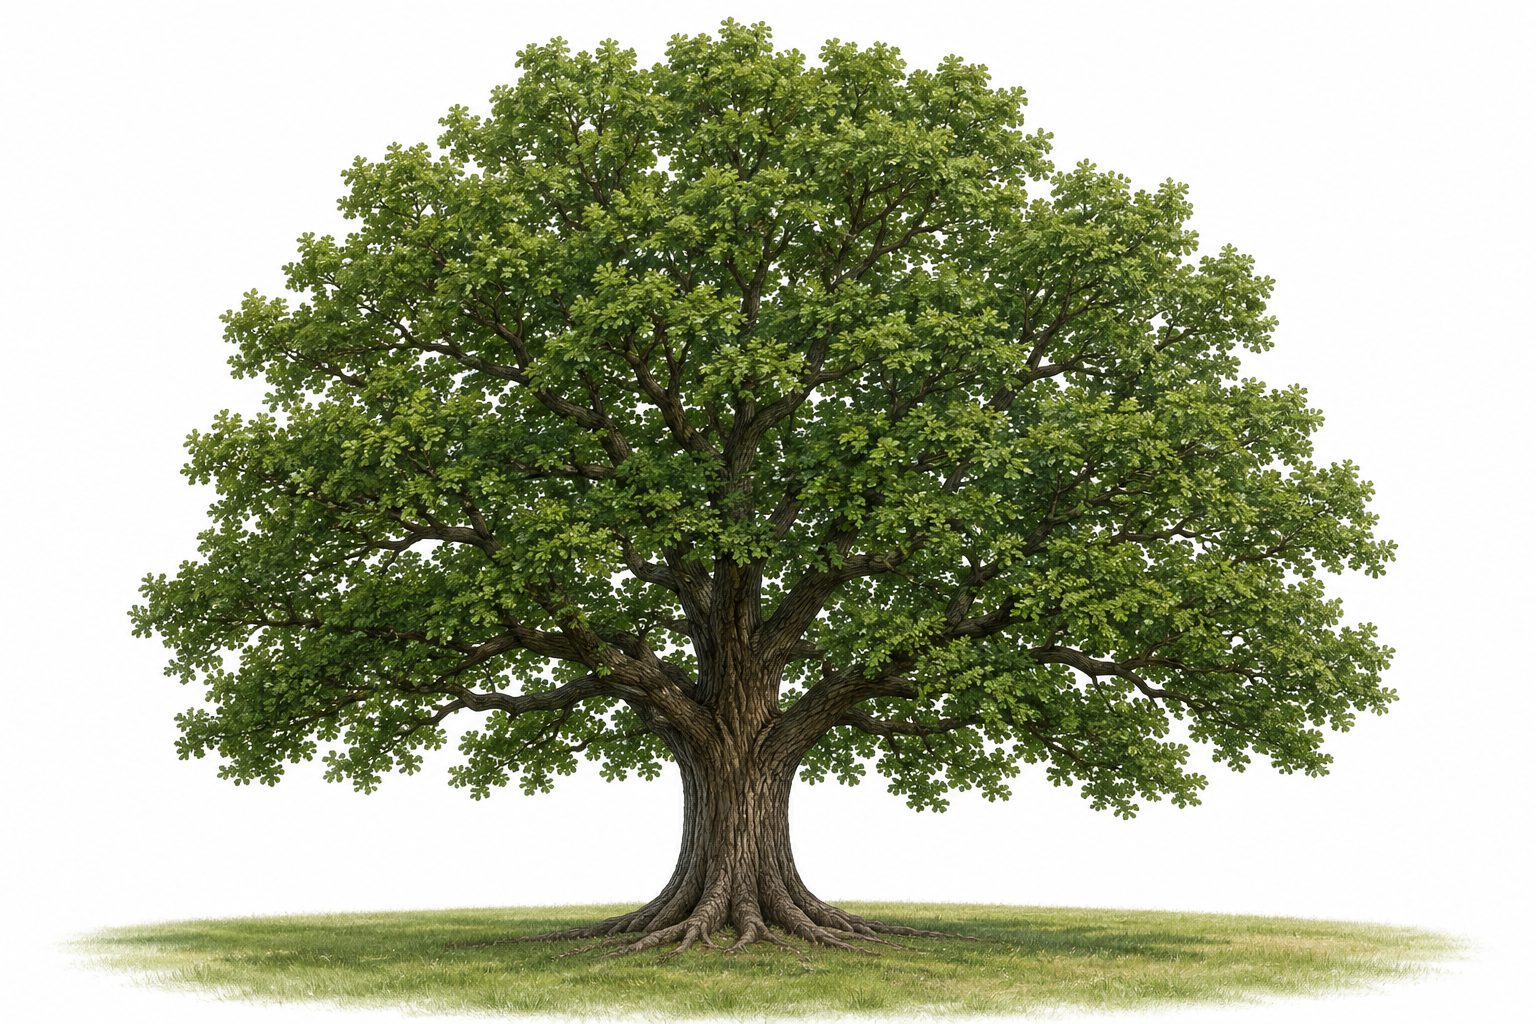
\includegraphics[width=0.62\linewidth]{images/book3/ai/b3-03-oak-tree.png}

{\small Un chêne isolé en été. Sa couronne est un assemblage de \omterm{def:b1:flowering-plant-organization:organs}{feuilles}
déployées pour intercepter la lumière~; le système racinaire, sous
l'herbe, est aussi large que la couronne et sa surface plusieurs fois
plus grande.}
\end{omfigure}

\section{L'appareil végétatif}

\begin{definition}[Racine, tige, feuille]\label{def:b1:flowering-plant-organization:organs}
L'\omterm{def:b1:mammal-organization:organ}{appareil} végétatif d'une plante à fleurs est fait de trois sortes
d'\omterm{def:b1:mammal-organization:organ}{organes}. La \emph{racine}\index{racine} ancre la plante et absorbe
l'eau et les ions minéraux du sol~; elle croît par son extrémité, se
ramifie, et porte des \emph{poils absorbants}\index{poil absorbant} juste
en arrière de la pointe. La \emph{tige}\index{tige} porte les feuilles
vers la lumière et conduit entre racines et feuilles~; elle est bâtie
d'unités répétées, chacune formée d'un \emph{nœud}\index{noeud@nœud} portant
une feuille et un bourgeon axillaire, et d'un
\emph{entre-nœud}\index{entre-noeud@entre-nœud} entre deux nœuds. La
\emph{feuille}\index{feuille} est l'\omterm{def:b1:mammal-organization:organ}{organe} de la photosynthèse~: un
limbe plat de grande surface et de faible épaisseur, porté par un
pétiole. Les racines forment le système racinaire~; tiges et feuilles,
le système caulinaire.
\end{definition}

\begin{proposition}[Un corps modulaire et ouvert]\label{prop:b1:flowering-plant-organization:modular}
Le corps de la plante est \emph{modulaire}\index{croissance modulaire}~:
la partie aérienne est une série d'unités identiques (nœud, \omterm{def:b1:flowering-plant-organization:organs}{feuille},
bourgeon, \omterm{def:b1:flowering-plant-organization:organs}{entre-nœud}) ajoutées l'une après l'autre par un bourgeon
apical, et chaque bourgeon axillaire peut engager une nouvelle série. La
croissance est \emph{indéfinie}\index{croissance indefinie@croissance indéfinie}~: il n'y a
pas de taille adulte, et la plante ajoute des modules, et donc de la
surface, aussi longtemps qu'elle vit. Le nombre et la disposition des
modules dépendent de la station --- lumière, eau, blessures --- de sorte
que la même espèce prend des formes différentes en des lieux différents.
Le corps d'un mammifère est au contraire clos~: ses \omterm{def:b1:mammal-organization:organ}{organes} sont en
nombre fixe et il cesse de croître à une taille déterminée.
\end{proposition}

\begin{omfigure}
\begin{tikzpicture}[font=\small, >=Stealth, line cap=round]
  % stem axis
  \draw[very thick, omExo!70!black] (0,0) -- (0,6.2);
  \node[circle, fill=omExo!70!black, inner sep=2.2pt] at (0,6.2) {};
  \node[right, font=\footnotesize, align=left] at (0.25,6.35) {bourgeon apical~: ajoute\\ de nouveaux modules au-dessus};
  % nodes with leaves and axillary buds
  \foreach \y/\side in {1.2/1, 2.6/-1, 4.0/1, 5.2/-1} {
    \fill[omExo!70!black] (0,\y) circle (2pt);
    \draw[thick, omExo!70!black] (0,\y) -- (\side*0.6,\y+0.25);
    \draw[thick, omExo, fill=omExo!30] (\side*0.6,\y+0.25) .. controls (\side*1.4,\y+0.6) and (\side*2.2,\y+0.15) .. (\side*2.0,\y-0.1) .. controls (\side*1.4,\y-0.25) and (\side*0.9,\y-0.05) .. (\side*0.6,\y+0.25);
    \fill[omProp] (\side*0.18,\y+0.28) circle (2pt);
  }
  % module bracket
  \draw[thick, gray] (-2.4,1.2) -- (-2.6,1.2) -- (-2.6,2.6) -- (-2.4,2.6);
  \node[left, font=\footnotesize, align=right, gray] at (-2.65,1.9) {un module~:\\ entre-nœud, nœud,\\ feuille, bourgeon axillaire};
  \node[right, font=\footnotesize] at (2.2,4.1) {feuille};
  \node[right, font=\footnotesize, omProp] at (0.25,2.95) {bourgeon axillaire};
  \node[left, font=\footnotesize] at (-0.3,3.3) {entre-nœud};
  \node[left, font=\footnotesize] at (-0.3,3.98) {nœud};
  % roots
  \draw[very thick, omDef!70!black] (0,0) -- (0,-1.6);
  \draw[thick, omDef!70!black] (0,-0.5) -- (-1.0,-1.3) (0,-0.9) -- (0.9,-1.5) (0,-1.2) -- (-0.5,-2.0);
  \foreach \x in {-0.12,-0.06,0.06,0.12} \draw[omDef!70!black] (\x,-1.55) -- (\x*3,-1.9);
  \node[right, font=\footnotesize, align=left] at (0.5,-0.75) {système racinaire~: croît par\\ les extrémités, poils absorbants derrière};
  \draw[dashed, gray] (-3.0,0) -- (3.2,0);
  \node[font=\footnotesize, gray, anchor=south east] at (3.2,0.02) {surface du sol};
\end{tikzpicture}

{\small La partie aérienne comme empilement de modules. Chaque nœud
porte une \omterm{def:b1:flowering-plant-organization:organs}{feuille} et un bourgeon axillaire~; le bourgeon apical ajoute
des modules au-dessus, et tout bourgeon axillaire peut engager un
rameau. Le système racinaire croît par ses extrémités.}
\end{omfigure}

\section{Les tissus de l'appareil primaire}

\begin{definition}[Tissus de revêtement, fondamentaux et conducteurs]\label{def:b1:flowering-plant-organization:tissues}
Tout \omterm{def:b1:mammal-organization:organ}{organe} de la plante est bâti de trois systèmes de tissus. Le
\emph{tissu de revêtement}\index{tissu de revetement@tissu de revêtement} est
l'\emph{épiderme}\index{epiderme@épiderme}, une assise unique de cellules
couvrant l'\omterm{def:b1:mammal-organization:organ}{organe}, enduite dans l'air d'une \emph{cuticule}\index{cuticule}
cireuse et percée de \emph{stomates}\index{stomate}, et prolongée dans
la \omterm{def:b1:flowering-plant-organization:organs}{racine} par les \omterm{def:b1:flowering-plant-organization:organs}{poils absorbants}. Le \emph{tissu
fondamental}\index{tissu fondamental} remplit l'\omterm{def:b1:mammal-organization:organ}{organe}~:
\emph{parenchyme}\index{parenchyme} (cellules vivantes à paroi mince,
pour la photosynthèse et les réserves),
\emph{collenchyme}\index{collenchyme} (cellules vivantes à paroi
inégalement épaissie, soutien souple des jeunes \omterm{def:b1:flowering-plant-organization:organs}{tiges}) et
\emph{sclérenchyme}\index{sclerenchyme@sclérenchyme} (cellules à paroi épaisse et
lignifiée, mortes à maturité, soutien rigide~: fibres et cellules
scléreuses). Le \emph{tissu conducteur}\index{tissu conducteur} conduit~:
le \emph{xylème}\index{xyleme@xylème} porte l'eau et les minéraux vers le haut
dans des \emph{trachéides}\index{tracheide@trachéide} et des
\emph{vaisseaux}\index{vaisseau} creux, lignifiés et morts
(\cref{ch:b1:plant-transport})~; le \emph{phloème}\index{phloeme@phloème} porte
les sucres dans des \emph{tubes criblés}\index{tube crible@tube criblé} vivants,
maintenus en vie par leurs cellules compagnes.
\end{definition}

\begin{omfigure}
\begin{tikzpicture}
  \node[anchor=south west, inner sep=0] (img) at (0,0)
    {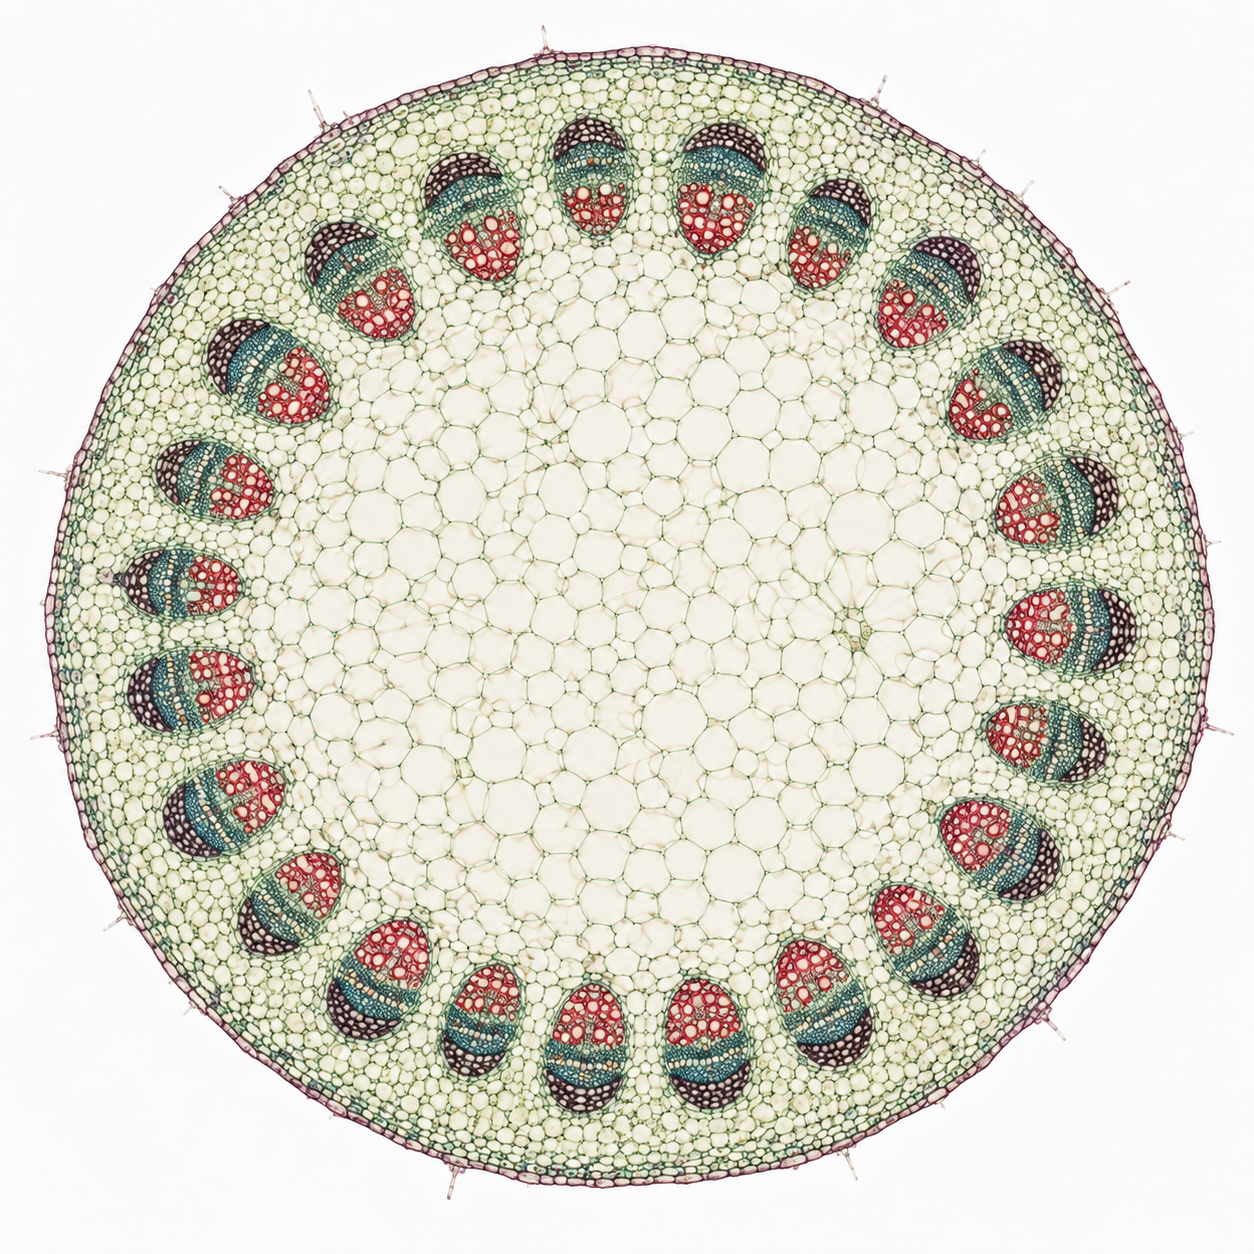
\includegraphics[width=0.5\linewidth]{images/book3/ai/fig-dicot-stem-cross.png}};
  \begin{scope}[x={(img.south east)}, y={(img.north west)},
      every node/.style={font=\small}]
    \draw[omDef, thick] (0.50,0.895) -- (0.50,1.06) node[above] {calotte de sclérenchyme d'un faisceau};
    \draw[omDef, thick] (0.87,0.50) -- (1.03,0.60) node[right] {phloème (vers l'extérieur)};
    \draw[omDef, thick] (0.81,0.50) -- (1.03,0.42) node[right] {xylème (vers l'intérieur)};
    \draw[omDef, thick] (0.50,0.50) -- (-0.03,0.50) node[left] {moelle};
    \draw[omDef, thick] (0.085,0.56) -- (-0.03,0.66) node[left] {cortex};
    \draw[omDef, thick] (0.06,0.40) -- (-0.03,0.32) node[left] {épiderme};
  \end{scope}
\end{tikzpicture}

{\small Coupe transversale d'une jeune \omterm{def:b1:flowering-plant-organization:organs}{tige} de dicotylédone. Les
faisceaux conducteurs forment un anneau~: dans chacun, le \omterm{def:b1:flowering-plant-organization:tissues}{xylème} (coloré
en rouge, lignifié) regarde le centre et le \omterm{def:b1:flowering-plant-organization:tissues}{phloème} l'extérieur, sous
une calotte de fibres. À l'intérieur de l'anneau, la moelle~; à
l'extérieur, le cortex et l'épiderme.}
\end{omfigure}

\begin{omfigure}
\begin{tikzpicture}
  \node[anchor=south west, inner sep=0] (img) at (0,0)
    {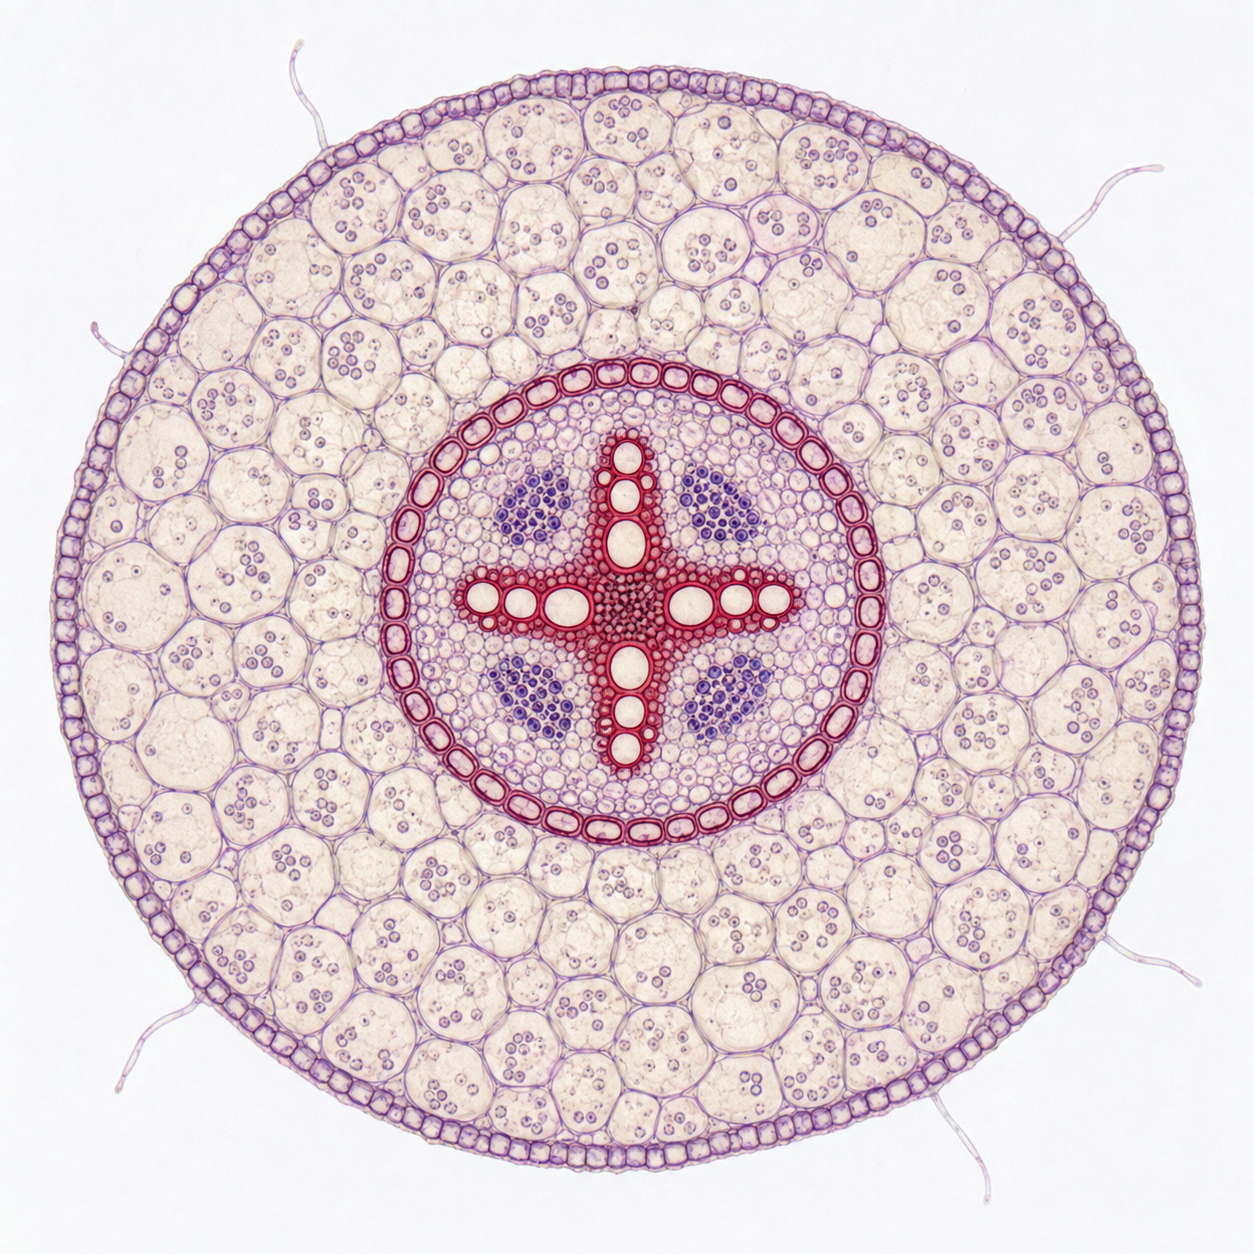
\includegraphics[width=0.46\linewidth]{images/book3/ai/fig-root-cross.png}};
  \begin{scope}[x={(img.south east)}, y={(img.north west)},
      every node/.style={font=\small}]
    \draw[omDef, thick] (0.50,0.52) -- (0.50,1.06) node[above] {étoile centrale de xylème};
    \draw[omDef, thick] (0.58,0.45) -- (1.03,0.38) node[right] {phloème entre les branches};
    \draw[omDef, thick] (0.695,0.50) -- (1.03,0.58) node[right] {endoderme};
    \draw[omDef, thick] (0.30,0.50) -- (-0.03,0.50) node[left] {cortex};
    \draw[omDef, thick] (0.06,0.62) -- (-0.03,0.74) node[left, align=right] {épiderme et\\ poils absorbants};
  \end{scope}
\end{tikzpicture}

{\small Coupe transversale d'une jeune \omterm{def:b1:flowering-plant-organization:organs}{racine} de dicotylédone. Un seul
cylindre conducteur central~: une étoile de \omterm{def:b1:flowering-plant-organization:tissues}{xylème} avec le \omterm{def:b1:flowering-plant-organization:tissues}{phloème} dans
les angles, bornée par l'endoderme~; autour, un large cortex~; à
l'extérieur, l'épiderme portant les \omterm{def:b1:flowering-plant-organization:organs}{poils absorbants}.}
\end{omfigure}

\begin{proposition}[Tige et racine diffèrent par la disposition des tissus conducteurs]\label{prop:b1:flowering-plant-organization:stemroot}
Dans la jeune \omterm{def:b1:flowering-plant-organization:organs}{tige}, les \omterm{def:b1:flowering-plant-organization:tissues}{tissus conducteurs} forment des faisceaux
disposés en anneau (dicotylédones) ou dispersés dans le \omterm{def:b1:flowering-plant-organization:tissues}{tissu
fondamental} (monocotylédones), chaque faisceau ayant le \omterm{def:b1:flowering-plant-organization:tissues}{xylème} vers le
centre et le \omterm{def:b1:flowering-plant-organization:tissues}{phloème} vers l'extérieur~; il n'y a pas d'endoderme, et le
\omterm{def:b1:flowering-plant-organization:tissues}{tissu fondamental} se partage entre une moelle centrale et un cortex
externe. Dans la jeune \omterm{def:b1:flowering-plant-organization:organs}{racine} il n'y a qu'un cylindre central~: le
\omterm{def:b1:flowering-plant-organization:tissues}{xylème} forme une étoile (deux à cinq branches chez les dicotylédones,
beaucoup chez les monocotylédones), le \omterm{def:b1:flowering-plant-organization:tissues}{phloème} se place entre les
branches, et le cylindre est borné par l'\emph{endoderme}\index{endoderme},
un anneau de cellules dont les parois radiales portent une bande
imperméable (\cref{ch:b1:plant-water-minerals}). La disposition suit la
fonction~: une \omterm{def:b1:flowering-plant-organization:organs}{tige} résiste à la flexion, et un anneau de faisceaux
près de sa surface est le plus rigide pour sa masse~; une \omterm{def:b1:flowering-plant-organization:organs}{racine} résiste
à la traction, et un cylindre central est la disposition d'un câble.
\end{proposition}

\begin{method}[Identifier une coupe végétale]\label{met:b1:flowering-plant-organization:section}
\begin{enumerate}
  \item Un unique cylindre conducteur central avec un endoderme~: une
        \omterm{def:b1:flowering-plant-organization:organs}{racine}. Des faisceaux en anneau ou dispersés, avec une moelle~:
        une \omterm{def:b1:flowering-plant-organization:organs}{tige}. Un \omterm{def:b1:mammal-organization:organ}{organe} aplati à deux épidermes et à couche
        lacuneuse~: une \omterm{def:b1:flowering-plant-organization:organs}{feuille}.
  \item \omterm{def:b1:flowering-plant-organization:organs}{Racine} à peu de branches de \omterm{def:b1:flowering-plant-organization:tissues}{xylème} (2--5)~: dicotylédone~;
        nombreuses branches autour d'une moelle~: monocotylédone. \omterm{def:b1:flowering-plant-organization:organs}{Tige} à
        faisceaux en un seul anneau~: dicotylédone~; faisceaux
        dispersés~: monocotylédone.
  \item Le \omterm{def:b1:flowering-plant-organization:tissues}{xylème} se reconnaît à ses cellules larges, à paroi épaisse et
        vides (rouges avec les colorants usuels)~; le \omterm{def:b1:flowering-plant-organization:tissues}{phloème} à ses
        petites cellules vivantes, \omterm{def:b1:flowering-plant-organization:tissues}{tubes criblés} et cellules compagnes
        (vertes ou bleues).
  \item Dans une coupe de \omterm{def:b1:flowering-plant-organization:organs}{tige}, le \omterm{def:b1:flowering-plant-organization:tissues}{xylème} regarde vers l'intérieur et le
        \omterm{def:b1:flowering-plant-organization:tissues}{phloème} vers l'extérieur. Dans une \omterm{def:b1:flowering-plant-organization:organs}{racine}, \omterm{def:b1:flowering-plant-organization:tissues}{xylème} et \omterm{def:b1:flowering-plant-organization:tissues}{phloème}
        alternent sur un même rayon.
\end{enumerate}
\end{method}

\begin{omfigure}
\begin{tikzpicture}
  \node[anchor=south west, inner sep=0] (img) at (0,0)
    {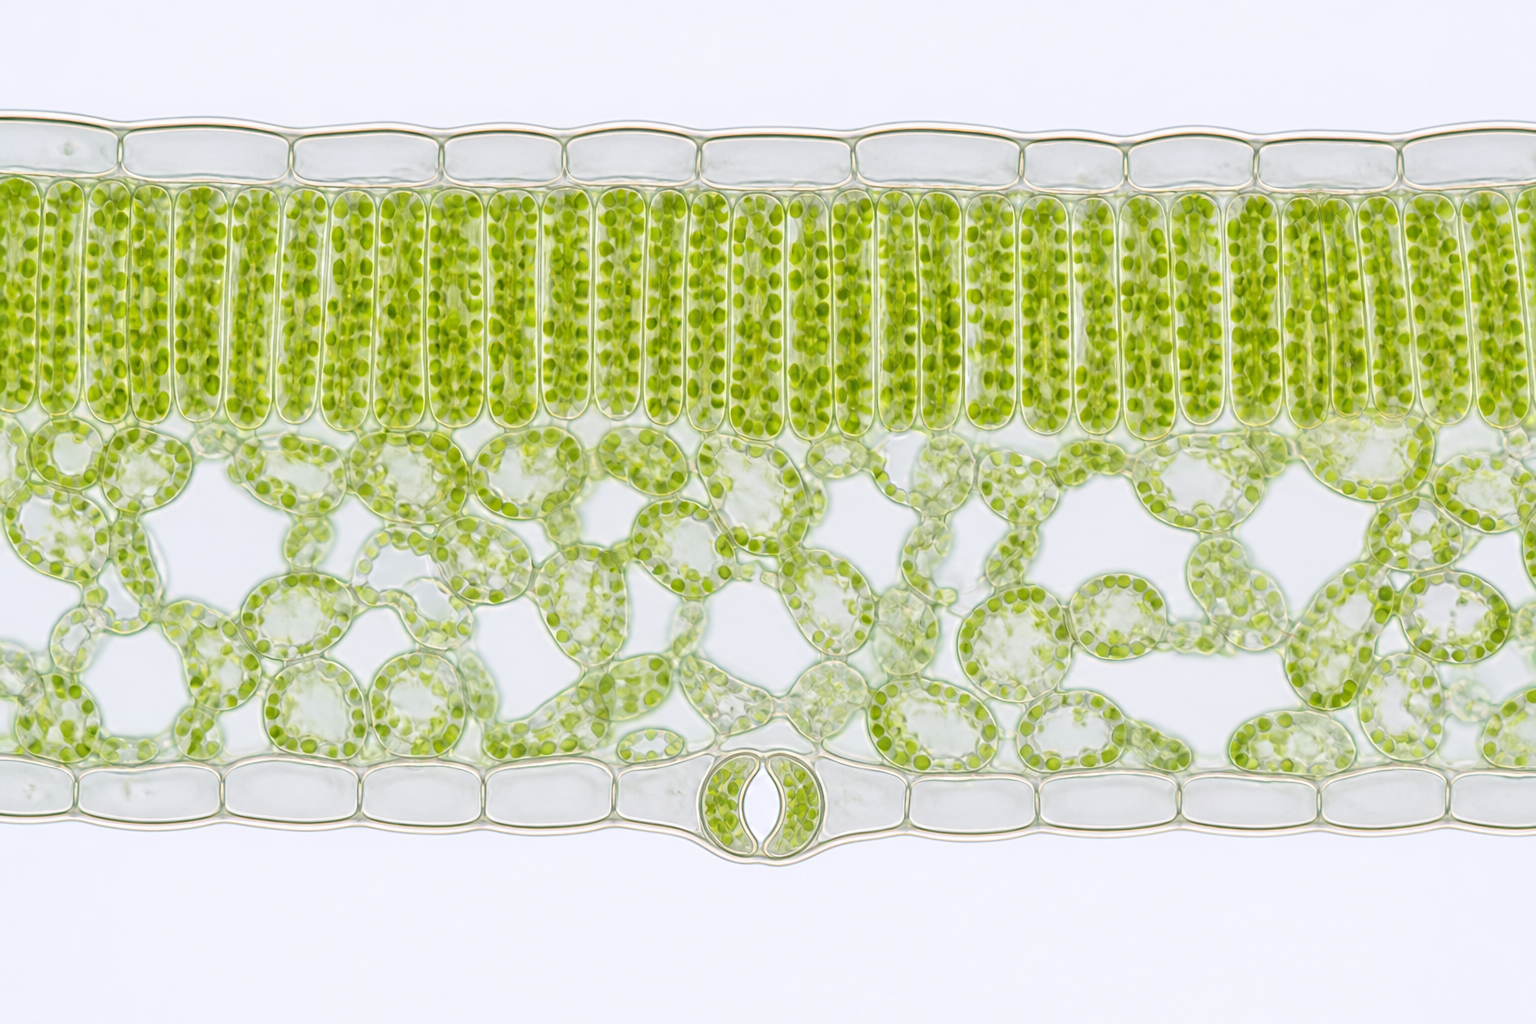
\includegraphics[width=0.48\linewidth]{images/book2/ai/fig-leaf-cross-section.png}};
  \begin{scope}[x={(img.south east)}, y={(img.north west)},
      every node/.style={font=\small}]
    \draw[omDef, thick] (0.50,0.94) -- (0.50,1.08) node[above] {épiderme supérieur, cuticule};
    \draw[omDef, thick] (0.30,0.70) -- (-0.03,0.80) node[left] {parenchyme palissadique};
    \draw[omDef, thick] (0.30,0.35) -- (-0.03,0.30) node[left] {parenchyme lacuneux};
    \draw[omDef, thick] (0.70,0.50) -- (1.03,0.60) node[right] {nervure};
    \draw[omDef, thick] (0.60,0.10) -- (1.03,0.10) node[right] {stomate};
  \end{scope}
\end{tikzpicture}

{\small Coupe transversale d'une \omterm{def:b1:flowering-plant-organization:organs}{feuille}. Entre les deux épidermes, les
cellules palissadiques en colonnes, bourrées de chloroplastes, font face
à la lumière, et les cellules lacuneuses lâches du dessous ménagent des
espaces d'air qui s'ouvrent par les \omterm{def:b1:flowering-plant-organization:tissues}{stomates}. Les nervures amènent l'eau
et emportent le sucre.}
\end{omfigure}

\begin{example}[Où se font les échanges]\label{ex:b1:flowering-plant-organization:where}
Le dioxyde de carbone entre dans une \omterm{def:b1:flowering-plant-organization:organs}{feuille} par ses \omterm{def:b1:flowering-plant-organization:tissues}{stomates}, traverse
les espaces d'air de la couche lacuneuse et se dissout dans les parois
humides des cellules palissadiques~; l'eau arrive par le \omterm{def:b1:flowering-plant-organization:tissues}{xylème} des
nervures et repart, sous forme de vapeur, par les mêmes \omterm{def:b1:flowering-plant-organization:tissues}{stomates}. L'eau
et les ions entrent dans la \omterm{def:b1:flowering-plant-organization:organs}{racine} par les \omterm{def:b1:flowering-plant-organization:organs}{poils absorbants} et
traversent le cortex jusqu'au \omterm{def:b1:flowering-plant-organization:tissues}{xylème} central. Les deux \omterm{def:b1:mammal-organization:organ}{organes} placent
leur \omterm{prop:b1:organism-environment:surfaces}{surface d'échange} à l'extérieur et leur \omterm{def:b1:flowering-plant-organization:tissues}{tissu conducteur} au milieu.
\end{example}

\section{La vie fixée~: les surfaces}

\begin{definition}[Indice foliaire]\label{def:b1:flowering-plant-organization:lai}
L'\emph{indice foliaire}\index{indice foliaire} $L$ d'un couvert végétal
est la surface foliaire totale, comptée sur une seule face, par unité de
surface de sol. Une prairie en juin a $L \approx 3$, une forêt
caducifoliée \qtyrange{4}{6}{}, une forêt tropicale humide jusqu'à
\qty{8}{}~: plusieurs épaisseurs de \omterm{def:b1:flowering-plant-organization:organs}{feuilles} sont empilées au-dessus de
chaque mètre carré de sol.
\end{definition}

\begin{proposition}[Interception de la lumière par un couvert]\label{prop:b1:flowering-plant-organization:beer}
La fraction de la lumière incidente qui atteint le sol sous un couvert
d'\omterm{def:b1:flowering-plant-organization:lai}{indice foliaire} $L$ décroît exponentiellement,
\[
\frac{I(L)}{I_0} = e^{-kL},
\]
avec un coefficient d'extinction $k$ compris entre $0.3$ (\omterm{def:b1:flowering-plant-organization:organs}{feuilles}
dressées) et $0.8$ (\omterm{def:b1:flowering-plant-organization:organs}{feuilles} horizontales), typiquement $0.5$. Un
couvert de $L = 5$ avec $k = 0.5$ intercepte
$1 - e^{-2.5} = \qty{92}{\%}$ de la lumière.
\end{proposition}
\begin{proof}
En descendant dans le couvert, chaque couche mince de surface foliaire
$\dd L$ intercepte une fraction $k\,\dd L$ de la lumière qui l'atteint,
$k$ étant la fraction de la surface horizontale ombrée par une unité de
surface foliaire (elle dépend de l'orientation des \omterm{def:b1:flowering-plant-organization:organs}{feuilles}). D'où
$\dd I = -kI\,\dd L$, dont la solution est l'exponentielle.
\end{proof}

\begin{omfigure}
\begin{tikzpicture}
\begin{axis}[
  width=0.86\linewidth, height=6.2cm,
  axis x line=bottom, axis y line=left,
  xmin=0, xmax=9, ymin=0, ymax=1.1,
  xlabel={indice foliaire $L$}, ylabel={fraction de lumière atteignant le sol},
  xlabel style={font=\small, at={(axis description cs:0.5,-0.12)}, anchor=north},
  ylabel style={font=\small},
  tick label style={font=\small}, xtick={0,2,4,6,8}, ytick={0,0.2,0.4,0.6,0.8,1.0},
  legend style={font=\small, at={(0.97,0.95)}, anchor=north east, draw=none},
  clip=false,
]
\addplot[very thick, omDef, domain=0:9, samples=60] {exp(-0.3*x)};
\addlegendentry{$k = 0.3$ (feuilles dressées, graminées)}
\addplot[very thick, omThm, domain=0:9, samples=60] {exp(-0.5*x)};
\addlegendentry{$k = 0.5$ (feuillu typique)}
\addplot[very thick, omProp, domain=0:9, samples=60] {exp(-0.8*x)};
\addlegendentry{$k = 0.8$ (feuilles horizontales)}
\draw[dashed, gray] (axis cs:5,0) -- (axis cs:5,0.082);
\node[font=\scriptsize, anchor=west] at (axis cs:5.3,0.36) {chêne, $L=5$~: \qty{8}{\%} restants};
\end{axis}
\end{tikzpicture}

{\small Lumière sous un couvert en fonction de l'\omterm{def:b1:flowering-plant-organization:lai}{indice foliaire}, pour
trois orientations de \omterm{def:b1:flowering-plant-organization:organs}{feuilles}. Au-delà de $L \approx 6$, une couche de
\omterm{def:b1:flowering-plant-organization:organs}{feuilles} supplémentaire n'apporte presque rien, ce qui explique que les
couverts s'arrêtent là.}
\end{omfigure}

\begin{proposition}[La surface racinaire dépasse la surface foliaire]\label{prop:b1:flowering-plant-organization:rootsurface}
Un unique plant de seigle cultivé quatre mois dans une caisse de
\qty{0.05}{m^3} de terre a produit \qty{620}{km} de \omterm{def:b1:flowering-plant-organization:organs}{racines}, de surface
\qty{240}{m^2}, et $\num{1.4e10}$ \omterm{def:b1:flowering-plant-organization:organs}{poils absorbants} représentant
\qty{400}{m^2} de plus~: une surface environ cent fois celle de ses
\omterm{def:b1:flowering-plant-organization:organs}{feuilles}, répartie dans le sol à raison de dix kilomètres de \omterm{def:b1:flowering-plant-organization:organs}{racine} par
litre. Les \omterm{def:b1:flowering-plant-organization:organs}{poils absorbants}, chacun étant le prolongement tubulaire
d'une cellule épidermique, large de \qtyrange{5}{20}{\micro m} et long
jusqu'au millimètre, sont le lieu de l'essentiel de l'absorption~; ils
vivent quelques jours et sont remplacés à mesure que la pointe avance.
\end{proposition}
\begin{proof}[Faits expérimentaux]
Dittmer (1937) a extrait de sa caisse le système racinaire entier d'un
plant de seigle, a compté et mesuré au microscope des échantillons de
chaque ordre de \omterm{def:b1:flowering-plant-organization:organs}{racine} et des \omterm{def:b1:flowering-plant-organization:organs}{poils absorbants}, puis a extrapolé~:
\qty{13.8}{} millions de \omterm{def:b1:flowering-plant-organization:organs}{racines} totalisant \qty{623}{km}, et \qty{14}{}
milliards de poils totalisant \qty{10620}{km}. L'eau et les minéraux du
sol se déplacent si lentement qu'une \omterm{def:b1:flowering-plant-organization:organs}{racine} doit se trouver à moins d'un
millimètre d'eux pour les prélever~; l'énorme longueur est ce qui place
une \omterm{def:b1:flowering-plant-organization:organs}{racine} à portée de chaque gouttelette.
\end{proof}

\begin{omfigure}
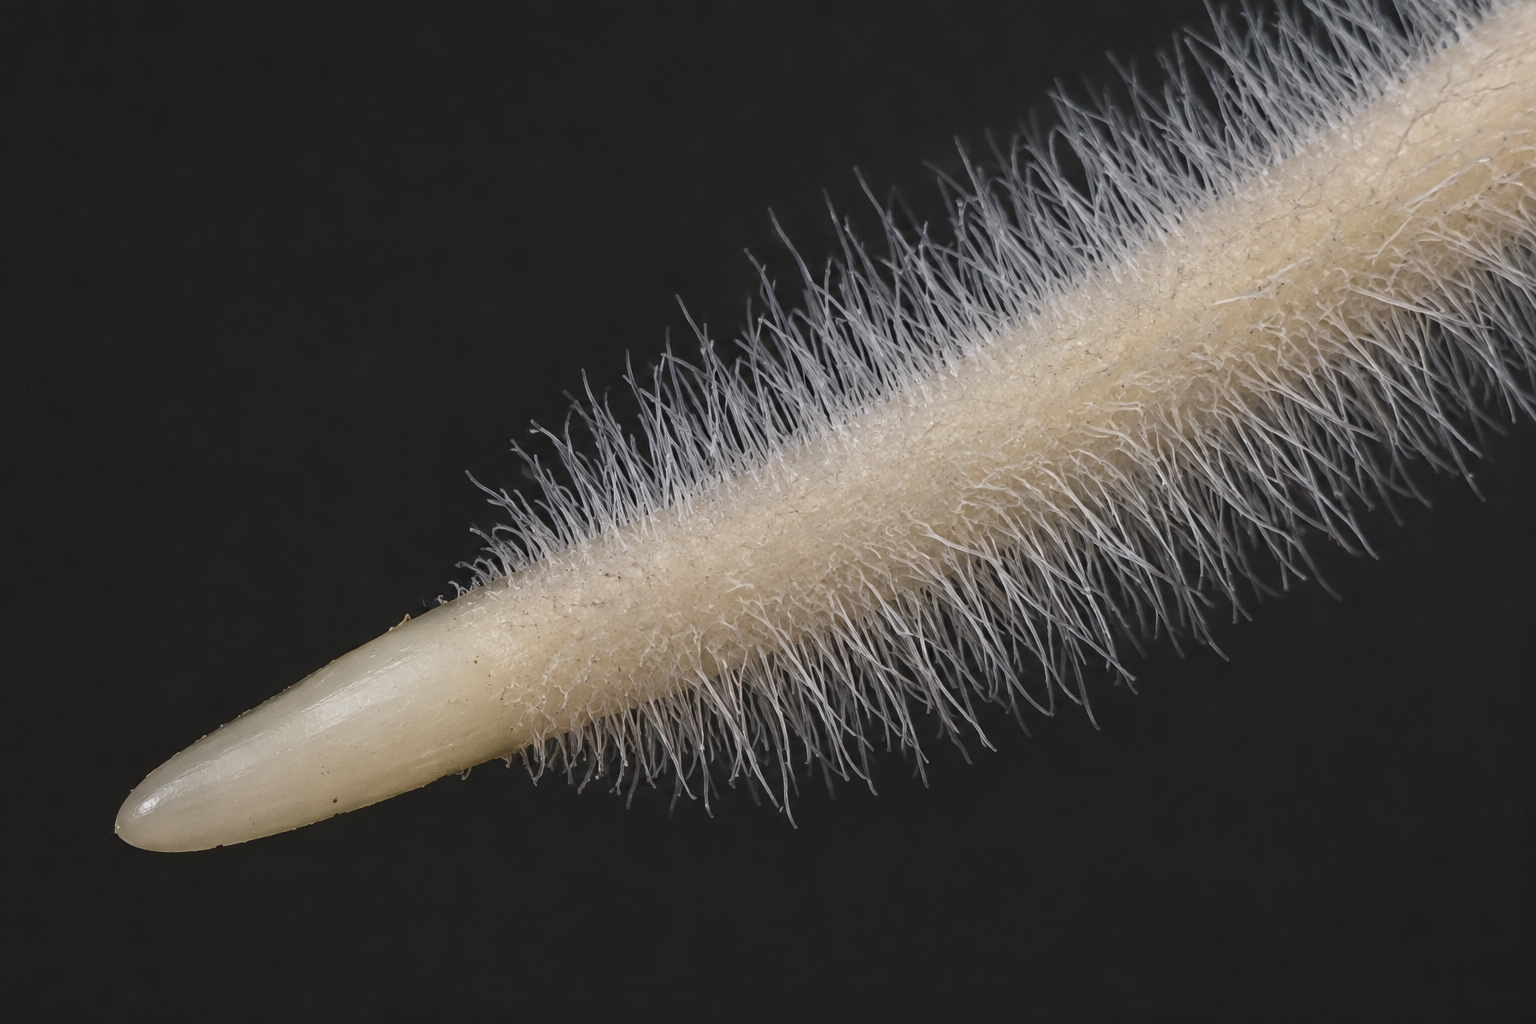
\includegraphics[width=0.58\linewidth]{images/book3/ai/b3-03-root-hairs.png}

{\small \omterm{def:b1:flowering-plant-organization:organs}{Poils absorbants} sur une plantule de radis, à quelques
millimètres en arrière de la pointe nue. Chaque poil est une unique
cellule épidermique allongée dans le sol~; ensemble ils multiplient
plusieurs fois la surface absorbante.}
\end{omfigure}

\begin{example}[Les deux surfaces du chêne]\label{ex:b1:flowering-plant-organization:oaksurfaces}
Un chêne dont la couronne ombre \qty{100}{m^2} à $L = 5$ porte
\qty{500}{m^2} de \omterm{def:b1:flowering-plant-organization:organs}{feuilles}. Ses \omterm{def:b1:flowering-plant-organization:organs}{racines} fines, à quelques kilomètres par
mètre cube dans \qty{100}{m^3} de sol, offrent plusieurs centaines de
mètres carrés, et leurs \omterm{def:b1:flowering-plant-organization:organs}{poils absorbants} un millier de plus~: la surface
absorbante souterraine vaut plusieurs fois la surface photosynthétique
aérienne, au-dessus des mêmes mètres carrés de sol.
\end{example}

\section{Croissance et forme}

\begin{definition}[Méristèmes, croissances primaire et secondaire]\label{def:b1:flowering-plant-organization:meristem}
Un \emph{méristème}\index{meristeme@méristème} est un tissu de petites cellules
indifférenciées qui continuent de se diviser. Les \emph{méristèmes
apicaux}\index{meristeme apical@méristème apical} des extrémités de chaque \omterm{def:b1:flowering-plant-organization:organs}{tige} et de
chaque \omterm{def:b1:flowering-plant-organization:organs}{racine} assurent la \emph{croissance
primaire}\index{croissance primaire}~: l'allongement, et les tissus
primaires ci-dessus. Les \emph{méristèmes
latéraux}\index{meristeme lateral@méristème latéral} --- le cambium entre \omterm{def:b1:flowering-plant-organization:tissues}{xylème} et
\omterm{def:b1:flowering-plant-organization:tissues}{phloème}, et le phellogène sous l'épiderme --- assurent la
\emph{croissance secondaire}\index{croissance secondaire}~:
l'épaississement, par ajout de bois (\omterm{def:b1:flowering-plant-organization:tissues}{xylème} secondaire) vers l'intérieur
et d'écorce vers l'extérieur, dans les \omterm{def:b1:flowering-plant-organization:organs}{tiges} et les \omterm{def:b1:flowering-plant-organization:organs}{racines} des arbres
et des arbustes. Les mécanismes de l'activité méristématique relèvent du
volume de deuxième année.
\end{definition}

\begin{omfigure}
\begin{tikzpicture}[font=\small, >=Stealth, line cap=round]
  % root outline (vertical, tip at bottom)
  \draw[thick, omDef!60!black, fill=omDef!8] (-0.7,5.2) -- (-0.7,1.3) .. controls (-0.7,0.4) and (-0.3,0) .. (0,-0.2) .. controls (0.3,0) and (0.7,0.4) .. (0.7,1.3) -- (0.7,5.2);
  % root cap
  \draw[thick, omDef!60!black, fill=omDef!25] (-0.72,0.9) .. controls (-0.75,0.2) and (-0.3,-0.35) .. (0,-0.45) .. controls (0.3,-0.35) and (0.75,0.2) .. (0.72,0.9) .. controls (0.5,0.55) and (0.2,0.4) .. (0,0.45) .. controls (-0.2,0.4) and (-0.5,0.55) .. (-0.72,0.9);
  % meristem
  \fill[omThm!45] (0,0.95) ellipse (0.45 and 0.35);
  % vascular strand
  \draw[thick, omDef!60!black, fill=omDef!30] (-0.15,5.2) -- (-0.15,1.9) .. controls (-0.1,1.5) .. (0,1.35) .. controls (0.1,1.5) .. (0.15,1.9) -- (0.15,5.2);
  % root hairs
  \foreach \y in {3.4,3.7,4.0,4.3,4.6,4.9} { \draw[omDef!60!black] (-0.7,\y) -- (-1.5,\y+0.15); \draw[omDef!60!black] (0.7,\y) -- (1.5,\y+0.15); }
  % zone brackets
  \draw[thick, gray] (2.0,-0.45) -- (2.2,-0.45) -- (2.2,0.6) -- (2.0,0.6); \node[right, align=left, font=\footnotesize] at (2.3,0.1) {coiffe~: protège la pointe,\\ perçoit la pesanteur};
  \draw[thick, gray] (2.0,0.6) -- (2.2,0.6) -- (2.2,1.4) -- (2.0,1.4); \node[right, align=left, font=\footnotesize] at (2.3,1.0) {zone de division~:\\ méristème apical (rouge)};
  \draw[thick, gray] (2.0,1.4) -- (2.2,1.4) -- (2.2,3.1) -- (2.0,3.1); \node[right, align=left, font=\footnotesize] at (2.3,2.25) {zone d'élongation~: les cellules\\ s'allongent d'un facteur dix et\\ poussent la pointe dans le sol};
  \draw[thick, gray] (2.0,3.1) -- (2.2,3.1) -- (2.2,5.2) -- (2.0,5.2); \node[right, align=left, font=\footnotesize] at (2.3,4.15) {zone de différenciation~:\\ poils absorbants, xylème et\\ phloème matures};
  \node[left, font=\footnotesize, align=right] at (-1.6,4.4) {poils absorbants};
  \node[left, font=\footnotesize, align=right] at (-0.85,2.4) {cylindre\\ conducteur\\ en formation};
\end{tikzpicture}

{\small Coupe longitudinale d'une extrémité de \omterm{def:b1:flowering-plant-organization:organs}{racine}. Derrière la
coiffe protectrice, le \omterm{def:b1:flowering-plant-organization:meristem}{méristème apical} se divise~; ses produits
s'allongent, puis se différencient en tissus de la \omterm{def:b1:flowering-plant-organization:organs}{racine} mature et
émettent des \omterm{def:b1:flowering-plant-organization:organs}{poils absorbants}. Toute la séquence occupe quelques
millimètres et progresse à mesure que la \omterm{def:b1:flowering-plant-organization:organs}{racine} croît.}
\end{omfigure}

\begin{proposition}[La forme suit la station]\label{prop:b1:flowering-plant-organization:plasticity}
Parce que sa croissance est modulaire et \omterm{prop:b1:flowering-plant-organization:modular}{indéfinie}, une plante façonne
son corps selon sa station (\emph{plasticité
phénotypique}\index{plasticite phenotypique@plasticité phénotypique})~: un arbre venu en terrain
découvert se ramifie bas et large, la même espèce en forêt élève un
tronc nu et haut~; une plante en sol sec consacre davantage de sa
croissance aux \omterm{def:b1:flowering-plant-organization:organs}{racines}, à l'ombre davantage aux \omterm{def:b1:flowering-plant-organization:organs}{feuilles}. Les espèces
des milieux secs (\emph{xérophytes}\index{xerophyte@xérophyte}) ont des \omterm{def:b1:flowering-plant-organization:tissues}{cuticules}
épaisses, des \omterm{def:b1:flowering-plant-organization:tissues}{stomates} enfoncés dans des cryptes ou protégés par des
poils, des \omterm{def:b1:flowering-plant-organization:organs}{feuilles} petites ou charnues et des \omterm{def:b1:flowering-plant-organization:organs}{racines} profondes~; les
espèces des milieux humides (\emph{hydrophytes}\index{hydrophyte}) ont
des \omterm{def:b1:flowering-plant-organization:tissues}{cuticules} minces, des \omterm{def:b1:flowering-plant-organization:tissues}{stomates} sur la face supérieure des \omterm{def:b1:flowering-plant-organization:organs}{feuilles}
flottantes, et un tissu rempli d'air
(\emph{aérenchyme}\index{aerenchyme@aérenchyme}) qui conduit l'oxygène jusqu'aux
\omterm{def:b1:flowering-plant-organization:organs}{racines} dans la vase anoxique.
\end{proposition}

\begin{example}[Mammifère et plante, côte à côte]\label{ex:b1:flowering-plant-organization:comparison}
Nutrition~: le mammifère mange de la matière organique~; la plante la
fabrique à partir de dioxyde de carbone, d'eau et de lumière. \omterm{prop:b1:organism-environment:surfaces}{Surfaces
d'échange}~: internes, de taille fixe, irriguées par le sang~; externes,
croissantes, ventilées par le vent et par le sol. \omterm{def:b1:organism-environment:milieu}{Milieu intérieur}~:
liquide régulé, de température et de composition constantes~; aucun ---
les cellules règlent leur propre contenu et la température de la plante
est celle de l'air. Croissance~: jusqu'à une forme adulte fixée~;
ouverte et modulaire, toute la vie durant. Mouvement~: l'animal va vers
sa nourriture~; la plante croît vers la lumière et vers l'eau.
Coordination~: nerfs et hormones, de la seconde à l'heure~; hormones
seules, de l'heure au jour. Chaque colonne est une manière cohérente
d'être un \omterm{def:b1:organism-environment:organism}{système ouvert}.
\end{example}

\section{Exercices}

\begin{exercise}[$\star$]\label{exo:b1:flowering-plant-organization:1}
Nommer les trois \omterm{def:b1:mammal-organization:organ}{organes} végétatifs d'une plante à fleurs et la
fonction principale de chacun.
\end{exercise}

\begin{exercise}[$\star$]\label{exo:b1:flowering-plant-organization:2}
Définir un module de la partie aérienne et expliquer ce que signifie
«~\omterm{prop:b1:flowering-plant-organization:modular}{croissance indéfinie}~».
\end{exercise}

\begin{exercise}[$\star$]\label{exo:b1:flowering-plant-organization:3}
Pour chaque tissu --- épiderme, \omterm{def:b1:flowering-plant-organization:tissues}{parenchyme}, \omterm{def:b1:flowering-plant-organization:tissues}{collenchyme}, \omterm{def:b1:flowering-plant-organization:tissues}{sclérenchyme},
\omterm{def:b1:flowering-plant-organization:tissues}{xylème}, \omterm{def:b1:flowering-plant-organization:tissues}{phloème} --- dire si ses cellules sont vivantes à maturité et
quel est son rôle.
\end{exercise}

\begin{exercise}[$\star$]\label{exo:b1:flowering-plant-organization:4}
D'après la figure de l'interception lumineuse, quelle fraction de la
lumière atteint le sol sous une prairie de $L = 3$ avec $k = 0.3$, et
sous une forêt de feuillus de $L = 6$ avec $k = 0.5$~?
\end{exercise}

\begin{exercise}[$\star\star$]\label{exo:b1:flowering-plant-organization:5}
Une coupe montre une étoile centrale de \omterm{def:b1:flowering-plant-organization:tissues}{xylème} à quatre branches, du
\omterm{def:b1:flowering-plant-organization:tissues}{phloème} entre les branches, un anneau de cellules à parois radiales
épaissies qui l'entoure, et une large zone de cellules arrondies à
l'extérieur. Identifier l'\omterm{def:b1:mammal-organization:organ}{organe} et le groupe, en donnant les deux
caractères qui décident de chacun.
\end{exercise}

\begin{exercise}[$\star\star$]\label{exo:b1:flowering-plant-organization:6}
Expliquer, à l'aide de la mécanique d'une poutre et de celle d'un câble,
pourquoi le \omterm{def:b1:flowering-plant-organization:tissues}{tissu conducteur} occupe un anneau périphérique dans la \omterm{def:b1:flowering-plant-organization:organs}{tige}
et un cylindre central dans la \omterm{def:b1:flowering-plant-organization:organs}{racine}.
\end{exercise}

\begin{exercise}[$\star\star$]\label{exo:b1:flowering-plant-organization:7}
Une culture a $L = 4$ et $k = 0.6$. Quelle fraction de la lumière
intercepte-t-elle~? De combien l'interception augmenterait-elle si $L$
passait à 6~? Commenter le rendement des \omterm{def:b1:flowering-plant-organization:organs}{feuilles} supplémentaires.
\end{exercise}

\begin{exercise}[$\star\star$]\label{exo:b1:flowering-plant-organization:8}
Le plant de seigle de Dittmer avait \qty{623}{km} de \omterm{def:b1:flowering-plant-organization:organs}{racines} et
\qty{240}{m^2} de surface racinaire. Calculer le diamètre moyen des
\omterm{def:b1:flowering-plant-organization:organs}{racines}. Si ses \omterm{def:b1:flowering-plant-organization:organs}{feuilles} totalisaient \qty{5}{m^2}, quel est le rapport
de la surface racines-plus-poils à la surface foliaire~?
\end{exercise}

\begin{exercise}[$\star\star$]\label{exo:b1:flowering-plant-organization:9}
Les \omterm{def:b1:flowering-plant-organization:organs}{poils absorbants} sont larges de $\qty{10}{\micro m}$ et longs de
$\qty{0.8}{mm}$, à raison de \qty{250}{} par millimètre de \omterm{def:b1:flowering-plant-organization:organs}{racine}. De
quel facteur multiplient-ils la surface d'une \omterm{def:b1:flowering-plant-organization:organs}{racine} de
$\qty{0.4}{mm}$ de diamètre~?
\end{exercise}

\begin{exercise}[$\star\star\star$]\label{exo:b1:flowering-plant-organization:10}
Un arbre en forêt a un tronc nu de \qty{20}{m} et une couronne réduite~;
la même espèce en plein champ est large et ramifiée dès \qty{2}{m}.
Expliquer les deux formes à partir de la \omterm{prop:b1:flowering-plant-organization:modular}{croissance modulaire} et du sort
des bourgeons axillaires à l'ombre et à la lumière, et dire ce que cette
plasticité coûte et ce qu'elle rapporte.
\end{exercise}

\begin{exercise}[$\star\star\star$]\label{exo:b1:flowering-plant-organization:11}
Une \omterm{prop:b1:flowering-plant-organization:plasticity}{xérophyte} a ses \omterm{def:b1:flowering-plant-organization:tissues}{stomates} enfoncés dans des cryptes tapissées de
poils. Expliquer ce que cela fait au gradient de vapeur d'eau entre les
espaces d'air de la \omterm{def:b1:flowering-plant-organization:organs}{feuille} et le vent, et ce que cela coûte en
absorption de dioxyde de carbone. Pourquoi est-ce un bon compromis dans
un désert et un mauvais dans une forêt humide~?
\end{exercise}

\begin{exercise}[$\star\star\star$]\label{exo:b1:flowering-plant-organization:12}
«~Une plante n'a pas de \omterm{def:b1:organism-environment:milieu}{milieu intérieur}.~» Discuter en un paragraphe~:
ce qui manque à la plante et que le mammifère possède, ce à quoi ses
cellules sont par conséquent exposées, et ce qu'elle fait à la place ---
surfaces, croissance, et la régulation qu'elle exerce tout de même.
\end{exercise}

\section{Problème~: les surfaces d'un chêne}

\begin{problem}[{Problème du week-end --- les feuilles d'un chêne
comptées en surface, ses stomates par milliards, son carbone et son eau
au kilogramme, et ses racines au kilomètre, jusqu'à la surface d'échange
qu'il déploie au-dessus de chaque mètre carré de son sol}]
\label{pb:b1:flowering-plant-organization:1}
La couronne d'un chêne ombre \qty{100}{m^2} de sol avec un \omterm{def:b1:flowering-plant-organization:lai}{indice
foliaire} $L = 5$ et un coefficient d'extinction $k = 0.5$. Ses faces
foliaires inférieures portent \qty{150}{} \omterm{def:b1:flowering-plant-organization:tissues}{stomates} par millimètre
carré~; un ostiole ouvert mesure \qty{10}{\micro m} sur
\qty{5}{\micro m}. En moyenne sur tout le couvert et sur une journée de
\qty{12}{h}, chaque mètre carré de \omterm{def:b1:flowering-plant-organization:organs}{feuille} absorbe
\qty{4}{\micro mol} de $\mathrm{CO_2}$ et perd \qty{1}{mmol} de vapeur
d'eau par seconde. Les \omterm{def:b1:flowering-plant-organization:organs}{racines} fines (diamètre \qty{0.5}{mm}) courent à
\qty{5}{km} par mètre cube dans \qty{1}{m} de profondeur de sol sous la
couronne~; les \omterm{def:b1:flowering-plant-organization:organs}{poils absorbants} (\qty{10}{\micro m} sur \qty{0.5}{mm})
poussent à \qty{200}{} par millimètre de \omterm{def:b1:flowering-plant-organization:organs}{racine} fine. Masses molaires~:
$\mathrm{CO_2}$ \qty{44}{g/mol}, C \qty{12}{g/mol},
$\mathrm{H_2O}$ \qty{18}{g/mol}.

\medskip
\noindent\textbf{Partie I --- \omterm{def:b1:flowering-plant-organization:organs}{Feuilles} et lumière.}
\begin{enumerate}
  \item Calculer la surface foliaire totale de la couronne, comptée sur
        une seule face.
  \item Calculer la fraction de lumière atteignant le sol et la
        fraction interceptée.
  \item Calculer la fraction interceptée si le chêne n'avait que
        $L = 2$, puis s'il avait $L = 8$.
  \item Expliquer à partir de ces nombres pourquoi un chêne s'arrête à
        $L \approx 5$.
  \item La \omterm{def:b1:flowering-plant-organization:organs}{feuille} moyenne mesure \qty{50}{cm^2}. Combien de \omterm{def:b1:flowering-plant-organization:organs}{feuilles} la
        couronne porte-t-elle~?
\end{enumerate}

\medskip
\noindent\textbf{Partie II --- \omterm{def:b1:flowering-plant-organization:tissues}{Stomates} et carbone.}
\begin{enumerate}[resume]
  \item Calculer le nombre de \omterm{def:b1:flowering-plant-organization:tissues}{stomates} de la couronne.
  \item Calculer la surface d'un ostiole ouvert et la fraction de la
        face foliaire inférieure que représentent les ostioles ouverts.
  \item Calculer l'absorption de $\mathrm{CO_2}$ de la couronne, en
        moles par seconde et en grammes par seconde.
  \item Calculer le $\mathrm{CO_2}$ absorbé en une journée de
        \qty{12}{h}, en kilogrammes, et le carbone qu'il contient.
  \item Sur une saison de végétation de \qty{150}{} jours, quelle masse
        de carbone la couronne fixe-t-elle~? Si la moitié est respirée
        par l'arbre lui-même, quelle masse de bois (\qty{50}{\%} de
        carbone) peut-il ajouter~?
\end{enumerate}

\medskip
\noindent\textbf{Partie III --- L'eau.}
\begin{enumerate}[resume]
  \item Calculer l'eau perdue par la couronne, en moles et en grammes
        par seconde.
  \item Calculer la perte d'eau quotidienne, en litres.
  \item Calculer le rapport du nombre de molécules d'eau perdues au
        nombre de molécules de $\mathrm{CO_2}$ gagnées. Pourquoi est-il
        si grand~?
  \item Une pluie de \qty{2}{mm} tombe sur les \qty{100}{m^2}. Combien
        de journées de transpiration couvre-t-elle, si toute cette eau
        atteint les \omterm{def:b1:flowering-plant-organization:organs}{racines}~?
\end{enumerate}

\medskip
\noindent\textbf{Partie IV --- Les \omterm{def:b1:flowering-plant-organization:organs}{racines}.}
\begin{enumerate}[resume]
  \item Calculer le volume de sol exploré et la longueur totale de
        \omterm{def:b1:flowering-plant-organization:organs}{racines} fines.
  \item Calculer la surface des \omterm{def:b1:flowering-plant-organization:organs}{racines} fines (assimilées à des
        cylindres).
  \item Calculer le nombre de \omterm{def:b1:flowering-plant-organization:organs}{poils absorbants}.
  \item Calculer la surface des \omterm{def:b1:flowering-plant-organization:organs}{poils absorbants}.
  \item Calculer la surface absorbante souterraine totale, et son
        rapport à la surface foliaire comptée sur une face.
  \item Les \omterm{def:b1:flowering-plant-organization:organs}{racines} fines sont à moins de \qty{1}{mm} de quelle fraction
        du volume de sol~? (Prendre chaque \omterm{def:b1:flowering-plant-organization:organs}{racine} pour l'axe d'un
        cylindre de rayon \qty{1}{mm}.)
  \item Comparer avec le plant de seigle du chapitre (\qty{620}{km} de
        \omterm{def:b1:flowering-plant-organization:organs}{racines} dans \qty{0.05}{m^3})~: laquelle des deux plantes
        explore son sol le plus complètement, et de quel facteur~?
  \item Additionner la surface foliaire comptée sur les deux faces et la
        surface racinaire. Diviser par les \qty{100}{m^2} de sol.
  \item Comparer avec le rapport, chez un humain, des \omterm{prop:b1:organism-environment:surfaces}{surfaces
        d'échange} repliées (\qty{130}{m^2}) à la surface externe
        (\qty{2}{m^2}).
  \item Expliquer en deux phrases pourquoi le rapport de la plante peut
        continuer de croître toute sa vie et pourquoi celui du
        mammifère ne le peut pas.
  \item Énoncer le résultat~: la \omterm{prop:b1:organism-environment:surfaces}{surface d'échange} qu'un chêne déploie
        par mètre carré de son sol, au-dessus et au-dessous, en mètres
        carrés.
\end{enumerate}
\end{problem}
